\appendix
\chapter{考前比记}

\begin{multicols}{2}
  \begin{itemize}
    \item \textbf{Repeating decimal to fraction}
    \begin{align*}
      x &= 0.62323... \\
      100x &= 62.323... \\
      100x - x &= 61.7 \\
      99x &= 61.7 \\
      x &= \frac{61.7}{99}
    \end{align*}

    \item \textbf{Big fraction to decimal}: take out as much powers of 10 as
    possible
    \begin{align*}
      x &= \frac{1}{2^{11} 5^{17}} \\
      &= \frac{1}{2^{11} 5^{11} 5^{6}} \\
      &= 10^{-11} \frac{1}{5^{6}}
    \end{align*}

    \item 1 is not a \textbf{prime number}
    \item All odd numebrs (ex. 1) behave the same; all even numbers
    (ex. 0) behave the same
    \item If \say{if A then opposite of B} is not true, then \say{if A then B}
    is true
    \begin{itemize}
      \item Ex. If \say{if $ w $ is even, then x must be odd} is not true, then
      \say{if $ w $ is even, then x must be even} is true
    \end{itemize}

    \item Items in \say{compared to} relationship can be reorganized as if they
    are in equality relationship
    \begin{equation}
      \frac{a}{b} \text{ compared to } c \to a \text{ compared to } bc
    \end{equation}

    \item A is three times half of B: $ A = \frac{3}{2} B $
    \item \textbf{Prime Number $ < $ 100}: 2, 3, 5, 7, 11, 13, 17, 19, 23, 29,
    31, 37, 41, 43, 47, 53, 59, 61, 67, 71, 73, 79, 83, 89, 97

    \item \textbf{Simple Interest}
    \begin{equation}
      V = P \left( 1 + \frac{tr}{100} \right)
    \end{equation}

    \begin{itemize}
      \item $ P $: principal
      \item $ t $: time
      \item $ r $: interest rate
    \end{itemize}

    \item \textbf{Compound Interest}: $ t $ is years
    \begin{itemize}
      \item \textbf{Compounded Once Per Year}
      \begin{equation}
        V = P \left( 1 + \frac{r}{100} \right)^{t}
      \end{equation}

      \item \textbf{Compounded $ n $ Times Per Year}
      \begin{equation}
        V = P \left( 1 + \frac{r}{100n} \right)^{nt}
      \end{equation}
      \begin{itemize}
        \item \textbf{Given the same interest rate, time and principal, the more
        often it is compounded, the higher the interest}
        \item \textbf{不能简化为}:
        \begin{equation}
          \text{profit } = P \left( \frac{r}{100n} \right)^{nt}
        \end{equation}
        因为本金每一次\say{compound}都在变
      \end{itemize}
    \end{itemize}

    \item \textbf{Wholesale vs Retail}
    \begin{itemize}
      \item \textbf{Wholesale}: 批发
      \item \textbf{Retail}: 零售
    \end{itemize}

    \item \textbf{Perpendicular}: 一线段斜率为 $ k $, 与之垂直的线段的斜率为
    $ -\frac{1}{k} $
    \item \textbf{图内三角形个数}
    \begin{equation}
      n - 2
    \end{equation}

    \item \textbf{边形的内角和公式}:
    \begin{equation}
      \left( n - 2 \right) \times 180
    \end{equation}

    \item \textbf{Congruent Triangle}
    \begin{itemize}
      \item 边边边
      \item 边角边
      \item 角边角
    \end{itemize}

    \item \textbf{Similar Triangle}:
    \begin{itemize}
      \item 两条边成比例, 夹角一样则相似
      \item \textbf{面积比为边长比的平方}
    \end{itemize}

    \item \textbf{Trapezoid (梯形) 面积}
    \begin{equation}
      S = \frac{1}{2}\left( b_{1} + b_{2} \right) \times h
    \end{equation}

    \item 当圆内接三角形有一边是直径的时候,该边对应的角为直角; 反之,当圆内接三角形有一
    个角为直角 时,该三角形必有一边为直径
    \item 同圆弧的圆周角相等
    \item 同圆弧的圆周角是圆心角的一半
    \item \textbf{Rhombus}: 菱形
    \begin{itemize}
      \item 所有边一样
    \end{itemize}

    \item \textbf{Weight}: the number of times a value appears in the list,
    or the frequency, is called the weight of that value

    \item \textbf{Weighted Sum}: when several values are repeated in a list,
    it is helpful to think of the mean of the numbers as a weighted mean of
    only those values in the list that are different. Weighted average=sum
    ($ \text{weight} \times \text{value} $)

    \item \textbf{Range}: the difference between the biggest and the smallest
    value

    \item \textbf{How to Find Quartiles}:
    \begin{enumerate}
      \item 先找 median, Q2
      \item median 左边的 median 为 Q1
      \item median 右边的 median 为 Q3
    \end{enumerate}

    \item \textbf{Interquartile Range}: Q1 to Q3; not influenced by outliers
    by outliers

    \item \textbf{Standardization}
    \begin{equation}
      \frac{x - \text{mean}}{\text{standard deviation}}
    \end{equation}

    \item \textbf{Influence of Change in Data}
    \begin{itemize}
      \item $ d \times x $: mean, median, mode, range, interquartile range,
      and standard deviation
      \item $ d - x $: mean, median, mode, range
    \end{itemize}

    \item \textbf{Relative Frequency}: frequencies that add up to $ 1 $
    \item \textbf{Percentile}: a value below which $ x \% $ of the data are
    placed
    \begin{itemize}
      \item Q1: $ 25\% $
      \item Q2: $ 50\% $
      \item Q3: $ 75\% $
    \end{itemize}

    \item \textbf{Standard Deviation}
    \begin{equation}
      \sqrt{\frac{\sum \left( x_{i} - \text{mean} \right)^{2}}{N}}
    \end{equation}
    \begin{itemize}
      \item Standard deviation测量数据和平均数的差距
    \end{itemize}

    \item \textbf{Multiplication Principal}: 当完成一件事是可以分步骤完成的,
    可以通过将每一步的possibilities相乘来计算完成该事件possibilities
    \item \textbf{Addition Principal}: 当完成一件事是可以分类完成的,可以通过将每一步
    的possibilities相加来计算完成该事件possibilities

    \item \textbf{Combination}: no order, no return
    \begin{equation}
      n C r = \frac{n!}{r! \left( n - r \right)!}
    \end{equation}
    \begin{itemize}
      \item $ n $: 总量
      \item $ r $: 所选量
    \end{itemize}

    \item \textbf{Permutation}: ordered, no return
    \begin{equation}
      n P r = \frac{n!}{\left( n - r \right)!}
    \end{equation}

    \item \textbf{Ordered, Returned}
    \begin{equation}
      n^{r}
    \end{equation}

    \item \textbf{Possibility}: 可能出现的结果
    \item \textbf{Probability}: 某种结果的概率
    \begin{align}
      P\left( A \cup B \right) &= P\left( A \right) + P\left( B \right) - P\left( A \cap B \right)
    \end{align}

    \item \textbf{Mutually Exclusive}
    \begin{align}
      P\left( A \cap B \right) &= 0
    \end{align}

    \item \textbf{Independence}:
    \begin{align}
      P\left( A \cap B \right) &= P\left( A \right) P\left( B \right)
    \end{align}

    \item \textbf{Round to nearest 0.05}: 0.05, 0.10, 0.15 ...
  \end{itemize}
\end{multicols}

\section{注意事项}

  \begin{itemize}
    \item $ x $的取值范围: $ x > 0, x < 0, x = 0 $?
    \item $ \sqrt{x}, x \ge 0 $
  \end{itemize}

\section{Distribution}

  \begin{figure}[H]
    \centering
    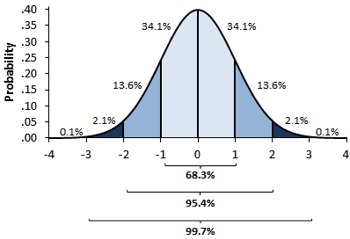
\includegraphics[width=\columnwidth]{images/remember-before-test/normal.jpg}
  \end{figure}

  \begin{itemize}
    \item x轴为$ \text{mean } + x \times \text{ standard deviation} $
  \end{itemize}

\section{3D 公式}

  \begin{figure}[H]
    \centering
    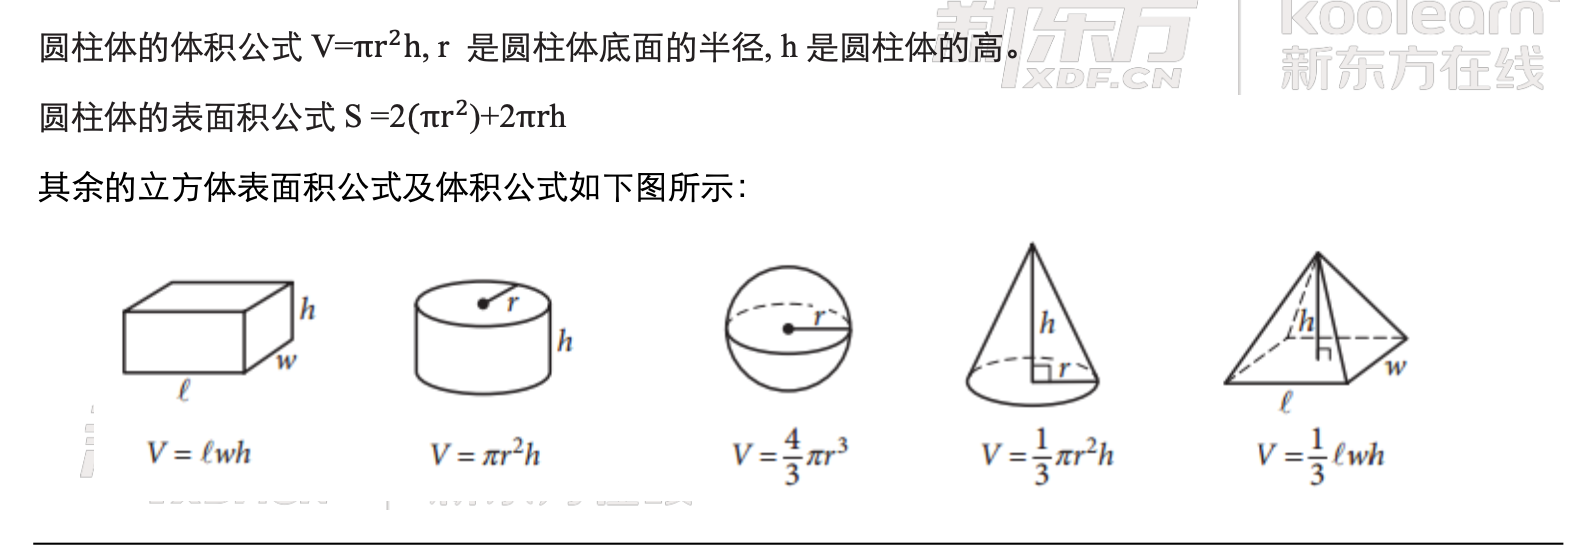
\includegraphics[width=\columnwidth]{images/remember-before-test/3d-equations.png}
  \end{figure}
